\section{PMFs and CDFs}

The \emph{probability mass function} (PMF) $p_X(a)$
of a random variable $X$ specifies the probability of
obtaining a number $X(\epsilon) = a$. We denote a PMF as
\begin{equation}
    p_X(a) = P[X = a]
\end{equation}
PMFs are represented with histograms.
\begin{figure}[h]
    \centering
    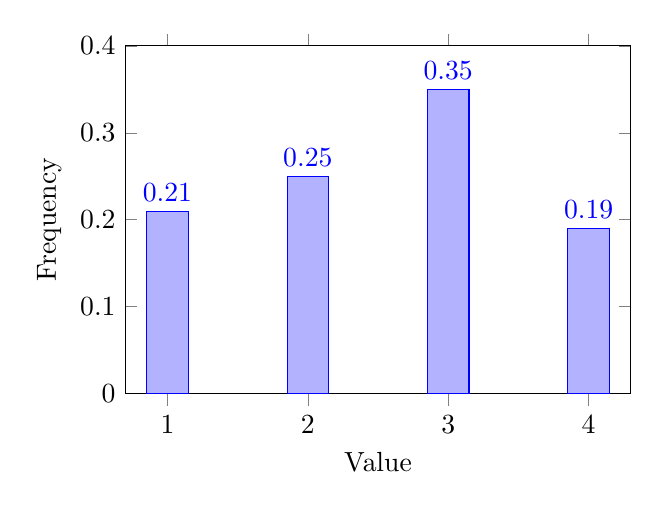
\begin{tikzpicture}
        \begin{axis}[
                ybar,
                bar width=15pt,
                xlabel={Value},
                ylabel={Frequency},
                xtick=data,
                ymin=0,
                ymax=0.4,
                nodes near coords,
                width=8cm,
                height=6cm
            ]
            \addplot coordinates {(1,0.21) (2,0.25) (3,0.35) (4,0.19)};
        \end{axis}
    \end{tikzpicture}
    \caption{PMF}
\end{figure}
A PMF should satisfy
\begin{equation}
    \sum_{x\in X(\Omega)} p_X(x) = 1
\end{equation}

The \emph{cumulative distribution function} is given by
\begin{align}
    F_X(x) & = P\left[X \leq x\right] \\
           & = \sum_{u \leq x} p_X(u)
\end{align}
and represents the sum of every impulse
of the PMF up to $x$.